\chapter{Experimenty}

\section{Druhy experimentů}

Experimenty začnu porovnáním náhodného hráče proti hráči využívajícím heuristiku pro rozhodování, dle \cref{sub:fantomai} a \cref{sub:detectivesai}. Lepší z těchto dvou hráčů, tj. ten který vyhraje více her, postoupí a odehraje další hry proti hráči, který využívá ISMCTS, dle mé implementace ze \cref{sec:impl}. Úvodní zápasy budou hrány v obou možnostech, tj. Fantom náhodný hráč proti detektivům s heuristikou a Fantom s heuristikou proti náhodným detektivům. Celý turnaj bude proveden na třech různých mapách.

Parametry hry jsou předem stanovené. Délka hry je 24 kol. Kola, kdy se Fantom musí ukázat jsou následující: 3., 8., 13., 18. a 21. Úvodní žetony každého detektiva jsou: drožka 10krát, taxi 9krát a tramvaj 5krát, úvodní žetony Fantoma jsou: drožka 
4krát, taxi 3krát a tramvaj 3krát. Všechny souboje provedu 50krát. V každém tahu má hráč s Monte Carlo technikami pro nalezení akce nastavenou délku simulování na 2,5 sekundy. Vyšší čas nabízí větší množství simulací, čímž by mohl být odhad nejlepší akce vylepšen. 

\section{Použité mapy}

Zvolené mapy, Obrázky \ref{fig:map1}, \ref{fig:map2} a \ref{fig:map3}, jsou náhodně vygenerované z implementace hry. Kvůli náhodnému generování mohou často vznikat mapy výhodné pro jednu stranu. Výběr map nedoprovázelo testování férovosti, experimenty popisují funkčnost v prostředí hry. 

\begin{figure}[h]
  \centering
  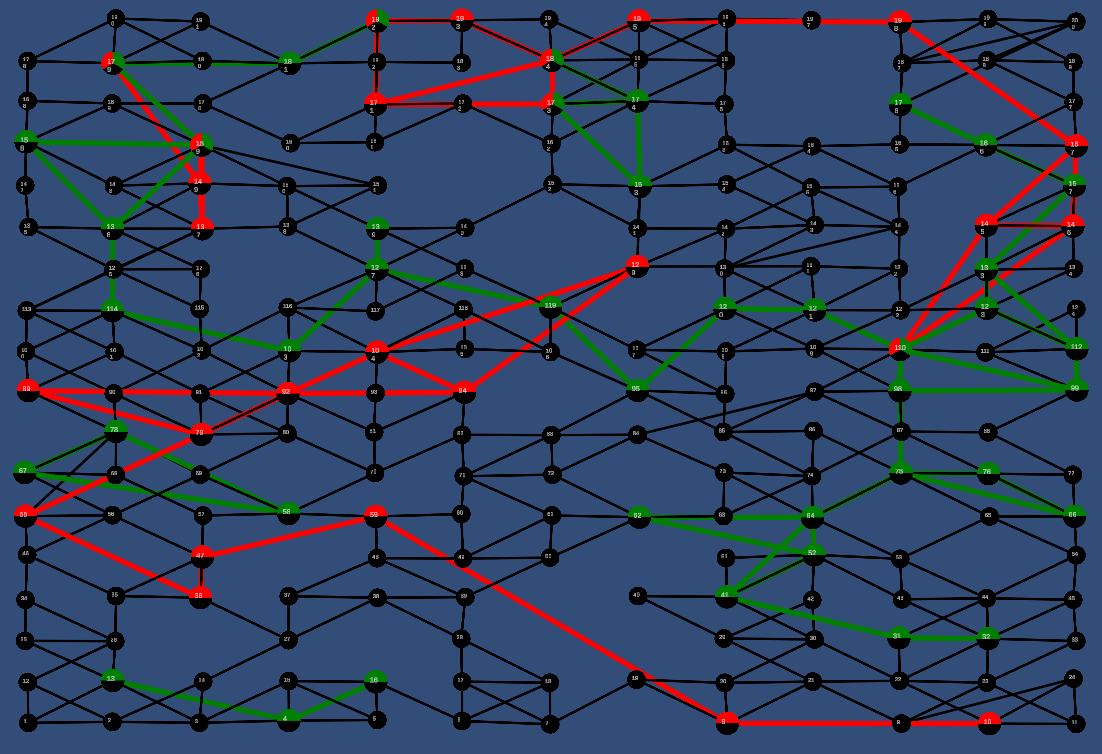
\includegraphics[width=1\textwidth]{mapa1.png}
  \caption{Mapa 1}
  \label{fig:map1}
\end{figure}

\begin{figure}[h]
  \centering
  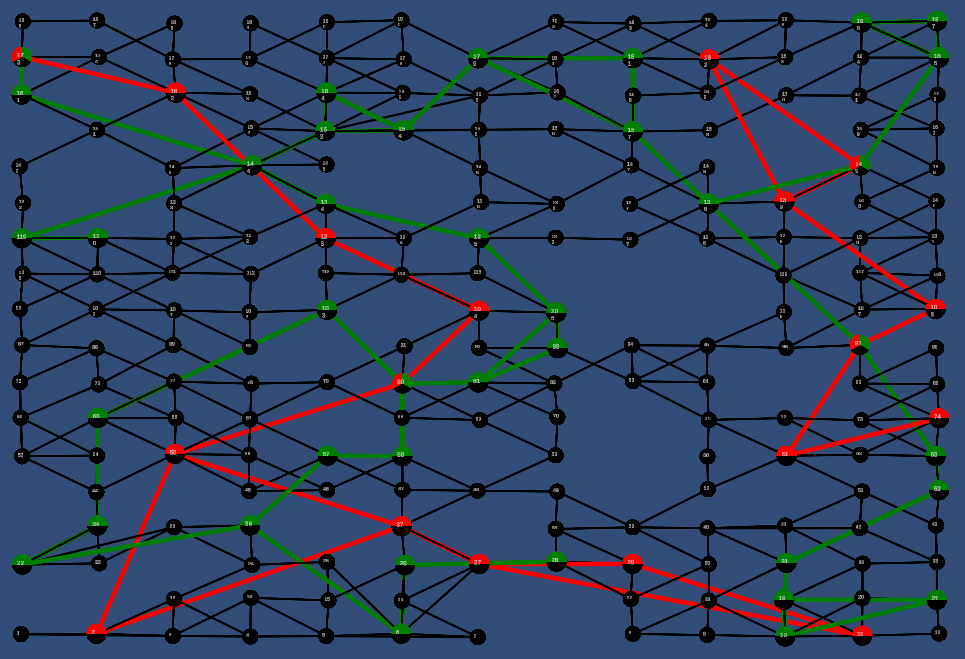
\includegraphics[width=1\textwidth]{mapa2.png}
  \caption{Mapa 2}
  \label{fig:map2}
\end{figure}

\begin{figure}[h]
  \centering
  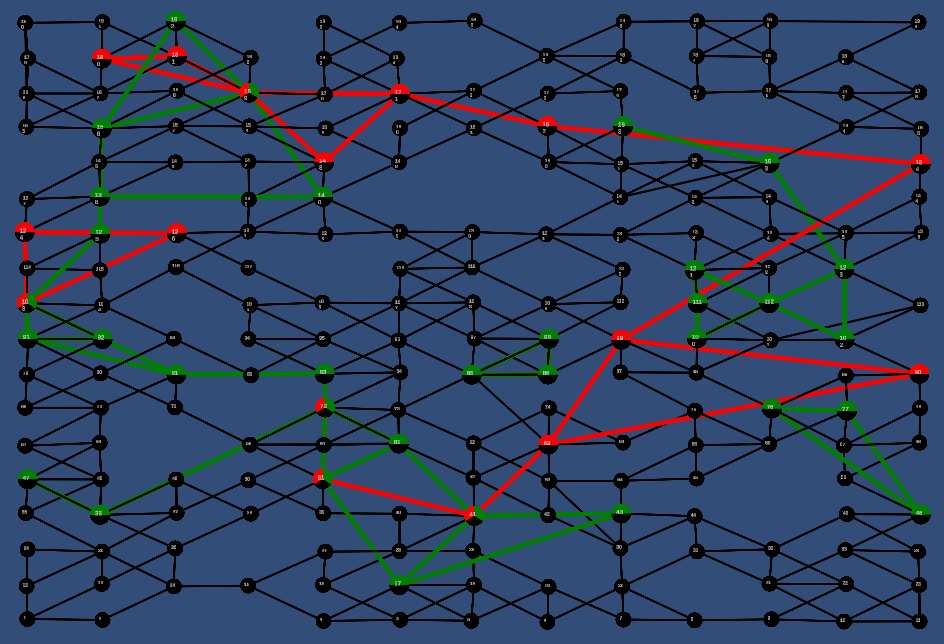
\includegraphics[width=1\textwidth]{mapa3.png}
  \caption{Mapa 3}
  \label{fig:map3}
\end{figure}
\clearpage

\section{Náhodný proti heuristice}
Nejdříve se proti sobě utkají náhodný hráč s hráčem využívající heuristiky dle \cref{sub:fantomai} a \cref{sub:detectivesai}. Náhodný hráč samozřejmě nijak nevyužívá znalosti a vlastnosti hry. Naopak hráč využívající heuristiku se snaží použít nejlepší možný tah s aktuálními znalostmi.

Z výsledků v tabulkách \ref{tab:heur-rand} a \ref{tab:rand-heur} je očividné, že se vyplatí využívat známé informace místo náhodného chození po mapě. Přesto se detektivům, kteří využívají heuristiku, daří proti náhodnému hráči více než Fantomovi. Detektivové s heuristikou neprohráli ani jednu hru. Důvodem nejspíše bude, že Fantom chce pro výhru využívat neznalosti detektivů, také náhodnými pohyby nijak netrestá vlastnosti heuristiky detektivů - směřují pouze k poslednímu známému místu Fantoma, jelikož se může zdržovat dlouze v blízkém okolí.

Na histogramech \ref{fig:hist-heur-rand} a \ref{fig:hist-rand-heur} je zobrazená četnost výherních kol z pohledů detektivů přes všechny tři testované mapy. 

Detektivové hrající náhodně proti chytřejšímu hráči využívající heuristiky, Obrázek \ref{fig:hist-heur-rand}, vyhrávali většinou díky náhodnosti prvního kola Fantoma - první tah volí čistě náhodně. V pozdějších kolech se díky heuristice Fantom mohl detektivům vyhýbat. Oproti tomu detektivové hrající dle heuristiky, Obrázek \ref{fig:hist-rand-heur}, nejčastěji vyhráli v prvních 12ti kolech. Heuristika je proti náhodnému hráči dostatečně silná, že náhodný Fantom skoro nikdy nevyhraje.

\begin{table}[htbp]
    \centering
    \caption{Počet výher detektivů (náhodný) a Fantoma (heuristika)}
    \label{tab:heur-rand}
    \begin{tabular}{@{}lcc@{}}
        \toprule
        \textbf{Mapa} & \textbf{Detektivové} & \textbf{Fantom} \\
        \midrule
        Mapa 1 & 9 & 41 \\
        Mapa 2 & 5 & 45 \\
        Mapa 3 & 4 & 46 \\
        \bottomrule
    \end{tabular}
\end{table}

\begin{table}[htbp]
    \centering
    \caption{Počet výher detektivů (heuristika) a Fantoma (náhodný)}
    \label{tab:rand-heur}
    \begin{tabular}{@{}lcc@{}}
        \toprule
        \textbf{Mapa} & \textbf{Detektivové} & \textbf{Fantom} \\
        \midrule
        Mapa 1 & 50 & 0 \\
        Mapa 2 & 50 & 0 \\
        Mapa 3 & 50 & 0 \\
        \bottomrule
    \end{tabular}
\end{table}

\begin{figure}[h]
  \centering
  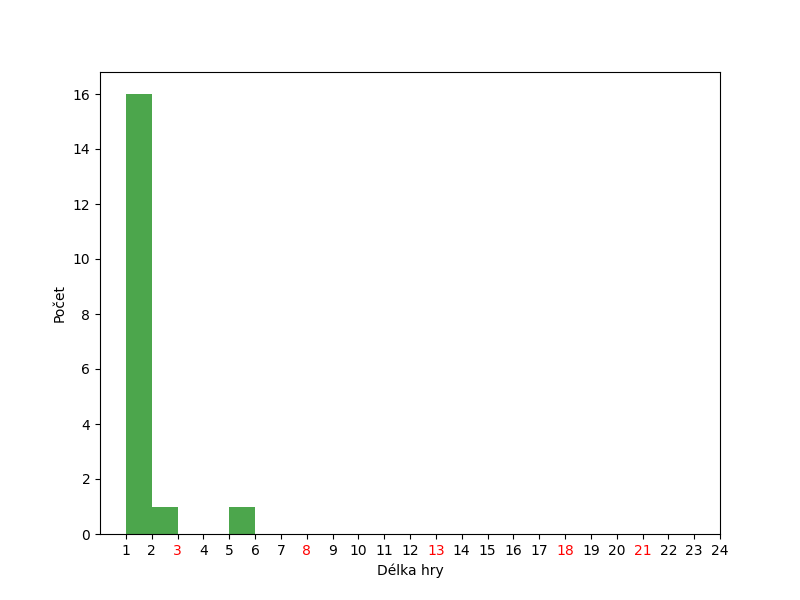
\includegraphics[width=0.85\textwidth]{heur-rand-histogram.png}
  \caption{Histogram délky her, kdy vyhráli detektivové. Fantom (heuristika) vs. detektivové (náhodný).}
  \label{fig:hist-heur-rand}
\end{figure}

\begin{figure}[h]
  \centering
  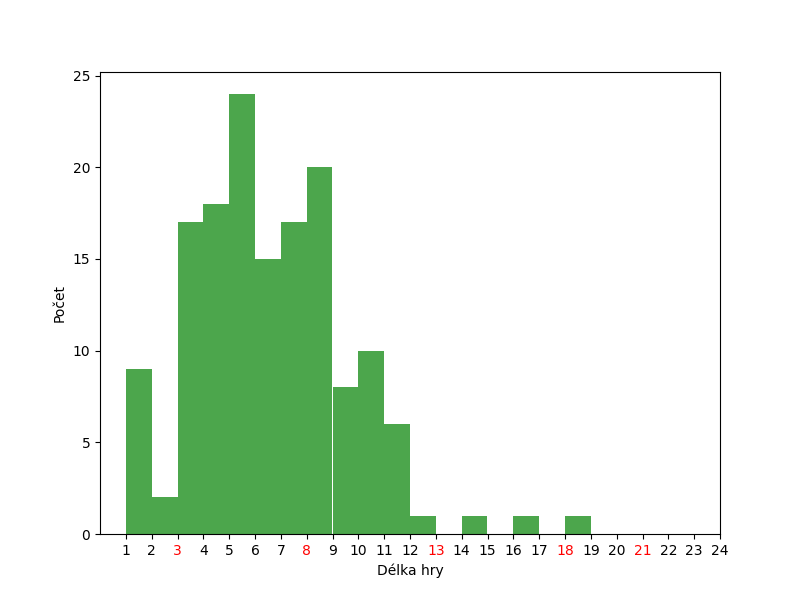
\includegraphics[width=0.85\textwidth]{rand-heur-histogram.png}
  \caption{Histogram délky her, kdy vyhráli detektivové. Fantom (náhodný) vs. detektivové (heuristika).}
  \label{fig:hist-rand-heur}
\end{figure}

\clearpage


\section{Heuristika proti ISMCTS}
Proti hráči využívající ISMCTS se utká hráč využívající heuristiku - výherce předešlého kola. Hráč se pomocí ISMCTS snaží simulovat průběhy her a ze simulací odvodit nejlepší tah.   

Na histogramech \ref{fig:hist-mcts-heur} a \ref{fig:hist-heur-mcts} je zobrazená četnost výherních kol z pohledů detektivů přes všechny tři testované mapy. 

Ve hrách, kdy Fantom využívá ISMCTS proti detektivům s heuristikou, Obrázek \ref{fig:hist-mcts-heur}, vychází, že detektivové nejčastěji vyhrají kolem poloviny délky hry - mezi 7. a 18. kolem. Oproti náhodnému Fantomovi trvá detektivům déle, než se jim podaří Fantoma dopadnout. Pokud se hra dostane do posledních kol, je možné, že detektivům také dochází žetony a přichází o možnosti dopadení Fantoma. Oproti tomu detektivové využívající ISMCTS proti Fantomovi s heuristikou hrají hůře, Obrázek \ref{fig:hist-heur-mcts}. Nejčastěji vyhrají díky náhodnému prvnímu kolu heuristiky, jinak v průběhu hry vyhrávají spíše ve druhé polovině.

\begin{table}[htbp]
    \centering
    \caption{Počet výher detektivů (heuristika) a Fantoma (ISMCTS)}
    \label{tab:mcts-heur}
    \begin{tabular}{@{}lcc@{}}
        \toprule
        \textbf{Mapa} & \textbf{Detektivové} & \textbf{Fantom} \\
        \midrule
        Mapa 1 & 17 & 33 \\
        Mapa 2 & 20 & 30 \\
        Mapa 3 & 19 & 31 \\
        \bottomrule
    \end{tabular}
\end{table}

\begin{table}[htbp]
    \centering
    \caption{Počet výher detektivů (ISMCTS) a Fantoma (heuristika)}
    \label{tab:heur-mcts}
    \begin{tabular}{@{}lcc@{}}
        \toprule
        \textbf{Mapa} & \textbf{Detektivové} & \textbf{Fantom} \\
        \midrule
        Mapa 1 & 4 & 46 \\
        Mapa 2 & 9 & 41 \\
        Mapa 3 & 2 & 48 \\
        \bottomrule
    \end{tabular}
\end{table}


\begin{figure}[h]
  \centering
  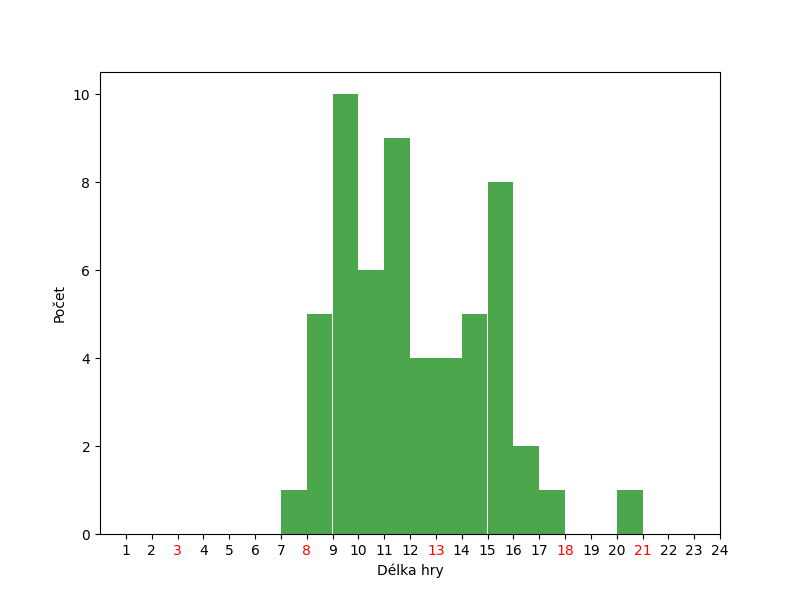
\includegraphics[width=0.85\textwidth]{mcts-heur-histogram.png}
  \caption{Histogram délky her, kdy vyhráli detektivové. Fantom (ISMCTS) vs. detektivové (heuristika).}
  \label{fig:hist-mcts-heur}
\end{figure}

\begin{figure}[h]
  \centering
  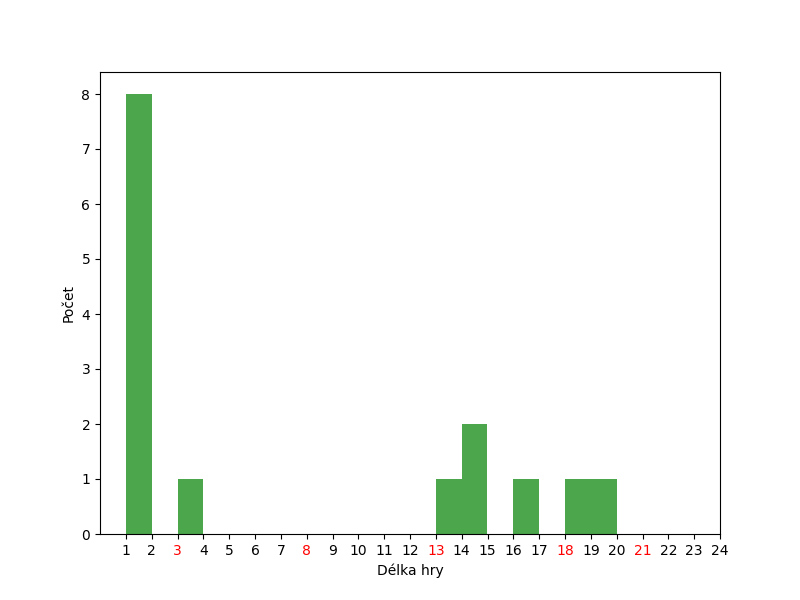
\includegraphics[width=0.85\textwidth]{heur-mcts-histogram.png}
  \caption{Histogram délky her, kdy vyhráli detektivové. Fantom (heuristika) vs. detektivové (ISMCTS).}
  \label{fig:hist-heur-mcts}
\end{figure}

Z výsledků v tabulkách \ref{tab:mcts-heur} a \ref{tab:heur-mcts} vyplývá, že Fantom využívající ISMCTS je lepší než hráč s heuristikou. Proti tomu, detektivové využívající ISMCTS dosahují velmi nízké úspěšnosti. Proti Fantomovi s heuristikou vyhrají méně než 10 \% her. 

Důvodů může být několik. Jedním z možných problémů je již zmíněný {\it strategy fusion} \cite{Soete2013MonteCarloTS}, který popisuje situaci, kde se algoritmus pokusí najít nejlepší strategii pro každou determinizaci zvlášť, místo hledání nejlepší strategie pro všechny determinizace zároveň. Proti Fantomovi používají detektivové 5 figurek, mají tedy řádově více možných akcí.

\clearpage
\section{Možná vylepšení ISMCTS}

Zlepšení algoritmu může poskytnout kvalitnější strategie, například se toho dá dosáhnout zefektivněním implementace algoritmu. Jiným způsobem je využít znalost domény hry. Zabudovat znalosti lze několika způsoby. Například je možné determinizace vybírat nikoliv uniformě z informačního stavu, ale podle pravděpodobnostní distribuce určující pravděpodobnost každého stavu. Pravděpodobnější determinizace budou častěji zvoleny a budou mít možnost více ovlivnit získanou strategii. Při iteraci je možné zvolit chytřejší simulační (rollout) strategii, která reprezentuje chování chytřejšího hráče místo náhodného.  

\section{Možná vylepšení heuristiky}
Zlepšení výsledků je možné dosáhnout upravením heuristiky pro první kolo. Kdyby v prvním kole nebyl výběr náhodný, bude hráč silnější. Například Fantom využívající heuristiky velmi často prohrál v prvním kole proti detektivům s~ISMCTS, histogram \ref{fig:hist-mcts-heur}.

\section{Závěr experimentů}
Vidíme, že mapy a parametry hry jsou nastaveny tak, že detektivové i Fantom mají naději na výhru. Záleží na jejich strategii a strategii oponenta. Navržení umělí hráči, využívající heuristiky či ISMCTS, poskytují škálu různě silných soupeřů pro lidského hráče.  
